\section{Evaluering}
\subsection{Test af Korrekthed}
Vi har som i \des løbende skrevet test før vi implementerede hver ny funktion i \code{RTP}-versionen.  Tabellen herunder viser testresultaterne for de test der er lavet specifikt for \code{RTP}-versionen.
\begin{longtable}{lr}
   	\toprule
    \mc{Test} & \mc{Resultat} \\
    \midrule
    \endfirsthead 
    \toprule
    \mc{Test} & \mc{Resultat} \\
    \midrule
    \endhead % slut efterfølgende headere
    \bottomrule
    \multicolumn{2}{r}{\textit{fortsættes}}
    \endfoot % slut footer
    \bottomrule
    \endlastfoot % slut sidste footer
test\_Alternation  & ok\\
test\_AlternationChoiseReader  & ok \\
test\_AlternationChoiseWriter  & ok \\
test\_AlternationExecuteReadDeadline  & ok\\
test\_AlternationExecuteSkipDeadline  & ok\\
test\_AlternationExecuteTimeoutDeadline  & ok \\
test\_AlternationExecuteWriteDeadline  & ok \\
test\_Alternationchoise1Deadline  & ok \\
test\_Alternationchoise2Deadline  & ok \\
test\_ChoisemultipleReader  & ok \\
test\_ChoisemultipleReader2  & ok \\
test\_ChoisemultipleWriter  & ok\\
test\_PoisonAndDeadline1  & ok\\
test\_PoisonAndDeadline2  & ok\\
test\_Reader\_Inheritance  & ok\\
test\_RetireAndDeadline  & ok\\
test\_Writer\_Inheritance  & ok\\
test\_channelpriority\_from\_low\_deadline  & ok\\
test\_channelpriority\_from\_low\_deadline2  & ok\\
test\_channelpriority\_from\_no\_deadline  & ok\\
test\_channelpriority\_from\_no\_deadline2  & ok\\
test\_readDeadline  &ok\\
test\_writeDeadline  & ok\\
test\_xreset\_inheritance  & ok\\
test\_xreset\_inheritance\_from\_two\_step  & FAIL\\
\end{longtable}


 Alle test med en undtagelse fungerer korrekt. Testen der fejler hedder test"_xreset"_inheritance"_from"_two"_step, og viser en situation hvor den samme proces får løftets sin prioritet to gange i træk, først med en høj prioritet, og efterfølgende med en mellemprioritet. Efterfølgende skal processen sænke sin prioritet, først til  mellemprioriteten og tilslut til sin originale prioritet. Her viser det sig vi har lavet en fejl i implementeringen, således at prioriteten ikke bliver nedsat til mellemprioriteten. \CRef{fig:priority-inheritance} viser prioriteten mens processen bliver op- og nedprioriteret. Tiden har ikke tilladt os at løse problemet, men  kan løses ved at kræve at, når en proces opprioriteres gemmes hvilken proces der står bag, så når en proces ønsker at fjerne sin opprioritering fra andre processer er det kun sin egen  prioritet den fjerner.  
 
  
\begin{figure}
 \begin{center}
  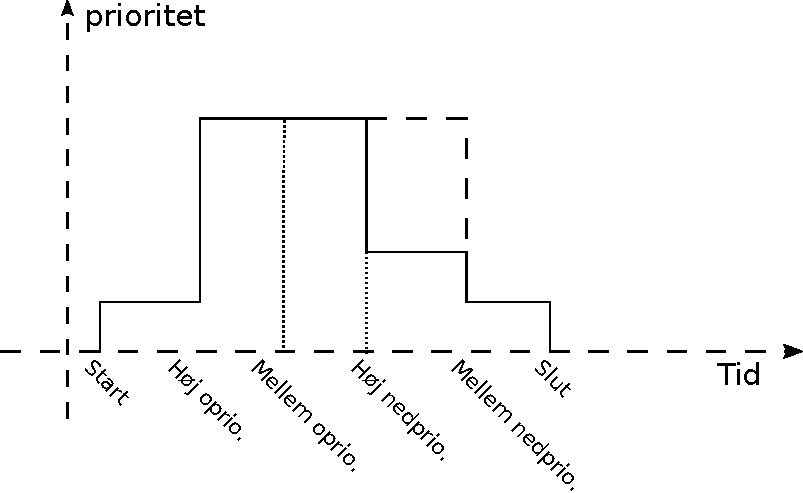
\includegraphics[scale=1]{images/priority-inheritance}
	\caption{Figuren viser hhv. forventet og faktisk prioritetsarvning. Der hvor den faktiske og forventede opførsel adskiller sig er forventet den fuldt optrukne streg, mens den stiplede streg er den faktiske opførsel.}
	\label{fig:priority-inheritance}
\end{center}
\end{figure}
  

\subsection{Slagterieksempel}

Først vil vi sammenligne de to udviklede versioner, for at se på deres fordele og ulemper, og til slut vi i dette afsnit sammenholde de to versioner, med et  eksempel der er implementeret i RTP-versionen.

Helt generelt opnår man når man ved brug af \pycsp et netværk, der nemt kan udvides hvis de fysiske rammer for slagteriet ændre sig. Viser det sig f.eks at kameraet holder den samlede produktivitet af netværket tilbage kan, slagteriet tilføjet endnu et kamera, og nemt udvide procesnetværket med endnu en kameraproces, som kan arbejde samtidigt med det første kamera. 

Forskellen i kode mellem \code{greenlets} og \code{proces}-versionen består af en linje, som indikerer hvilken version \pycsp skal bruge. En kørsel mellem de to versioner giver dog forskelligt resultat, som vist i \cref{tab:deadline-runs}. Dermed har valget af version betydning for både andelen af griseobjekter, der kan nå at blive bearbejdet, og hvor lang tid det tager i køre testen. Dette skyldes at testen køres på en multikerne CPU hvor \code{proces}-versionen dermed har mulighed for at køre parallelt. \code{Greenelts}-versionen derimod er begrænset til kørsel af en proces hvorfor der er flere grise der ikke når at blive bearbejdet inden for sin deadline.

\begin{table}[htbp]
	\centering
	\begin{tabular}{lrr}
       	\toprule
        \mc{Version} & \mc{Succesrate (\%)} & \mc{Tidsforbrug (s)} \\
        \midrule
        Greenlets & 42 & 16,5\\
        Processes & 71 & 10,3\\
        \bottomrule
    \end{tabular}
	\caption[]{Gennemførslen af simulation hvor 100 grise bliver sendt igennem procesnetværket. }\\
	\label{tab:deadline-runs}
\end{table}

Forskellen på kørselstiderne skyldes at detektoren venter på at aflevere griseobjektet til kameraet, og først når objektet er afleveret venter detektoren et normalfordelt tidsrum. Om dette er en urealistisk opførsel vil kræve mere domæneviden. Kan detektoren f.eks styre transportbåndet der fører grisene hen til detektoren er det en rimelig antagelse, mens det er urealistisk hvis båndet kører uafhængigt at detektoren.

I \code{procees}-versionen findes der fire processer og dermed kan der bearbejdes fire griseobjekter samtidigt. Dette sikre at det er de fire  griseobjekter nærmest robotten der arbejdes på, men samtidigt betyder det at man maksimalt kan arbejde på fire grise samtidigt. Ved at øge antallet af griseobjekter man kan arbejde på, vil man få mere tid per gris til at foretage de nødvendige beregninger. Man kan derfor vælge at tilføje flere konverterings og analyseprocesser, da disse ikke er bundet op på specialiseret hardware, og på den måde øge antallet af processer der kan arbejde samtidigt. Dette vil dog øge antallet af processer der må kæmper mod hinanden for CPU-tid, og griseobjekterne vil desuden skulle kæmpe mod hinanden for at komme igennem netværket uden hensyn til hvilken gris der er nærmest robotten. Man risikere dermed en starvation situation hvor griseobjekter svarende til  grise længere tilbage på transportbåndet overhaler griseobjekter længere fremme på transportbåndet.

\code{RTP}-udvidelsen bygger på \code{greenlets}-versionen, og vil derfor have de samme begrænsninger som denne, som diskuteret i implementeringen i afsnit \cref{sec:deadline-exampel-implementation}. Der er dog også en række fordele som vi vil komme ind på her.

Ved implementering af slagterieksemplet i \code{RTP}-versionen, slipper de enkelte processer for at holde styr på tiden, og vurdere om den enkelte gris deadline er overskredet. Når de modtager en gris sætter de deres egen deadline til grisens via funktionen \code{Set\_deadline}.  Hver proces skal i modsætningen til \code{greenlets}-versionen, kunne håndtere at modtage en \code{DeadlineException}, som de i dette eksempel blot kan håndteres ved at smide den nuværende griseobjekt væk. Det kan de gøre, da robotten på dette tidspunkt tager en beslutning uden specialviden om grisen, og griseobjektet er derfor ikke længere er relevant. I stedet kan processen  gå i gang med modtage et nyt griseobjekt.

I \code{greenlets}-versionen kom vi ind på at processerne frivilligt skal afgive kontrollen, før robotten kan foretage udskæringen, men at der ikke findes en metode til midlertidigt at afgive kontrollen. Med \code{RTP}-versionen og funktionen \code{Release} har alle processer mulighed for at afgive kontrollen så robotten rettidigt kan foretage selve udskæringen. Hermed skal vi ikke introducere en delt datastruktur.
  
selvom det var nødvendigt at basere RTP på  \code{greenlets}-versionen, medfører det at  kun en proces kan være aktiv på samme tid. Dermed kan vi kun udnytte en processor, som  passer dårligt sammen med denne applikation, som det ses af \cref{tab:deadline-runs}.  Vi kan dog til dels afhjælpe dette problem ved at udnytte at der i \code{greenlets}-versionen, findes en \code{IO}-dekorering. Denne dekorering placerer en funktion i en separat tråd, så flere funktioner kan køre samtidigt. Man skal her dog være opmærksom på at GIL'en stadig forhindre parallel udførsel. Eventuel parallel udførsel vil derfor kræve at koden i IO dekoreringen, kalder eksterne moduler som diskuteret i \cref{chap:csp}. Denne mulighed for parallel bearbejdning af flere processer vil dog  som i \code{processes}-versionen resultere i at processerne vil kæmpe mod hinanden om CPU-resurser. \code{RTP}-versionen har dog den store fordel at vi sikrer vi i modsætning til \code{proces}-versionen ikke risikere at griseobjekterne overhaler hinanden, men at netværket hele tiden har fokus på først at videresende griseobejektet nærmest robotten. \CRef{fig:pig-network3} viser hvordan netværket kan se ud med flere konverterings og analyse processer. 

\begin{figure}
 \begin{center}
  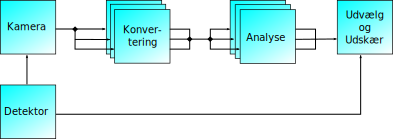
\includegraphics[scale=1]{images/pig-network3}
	\caption{Procesnetværk med flere konverteringsprocesser, og analyseprocesser}
	\label{fig:pig-network3}
\end{center}
\end{figure}
